\section{基础设施}\label{infrastructure}

Kimi K3 在一个模型中同时应对了三类罕见叠加的系统挑战：混合 KDA 注意力、3T 级稀疏多模态训练与推理，以及百万 Token 的智能体工作负载。我们的基础设施围绕这些挑战，在模型全生命周期中进行了协同设计。在架构层面，高性能 KDA Kernel 和上下文并行性使得循环公式在设备内部和跨设备间都能高效执行，覆盖训练与推理。在预训练阶段，均衡的专家执行、降低的内存占用以及通信重叠调度保证了大尺度下的高利用率。在百万 Token 智能体强化学习阶段，分层状态管理和可恢复的沙箱执行在多次迭代间保留了长轨迹。最后，状态感知的 KDA 前缀缓存、专用推理 Kernel 以及缓存与预算感知的调度将这些效率优势转化为可预测的生产服务。

\subsection{KDA 的算法-系统协同设计}\label{algorithm-system-co-design-for-kda}

KDA 将 softmax 注意力中不断增长的 key--value 缓存替换为固定大小的循环状态 \(\mathbf { S } \in \mathbb { R } ^ { d _ { k } \times d _ { v } }\)（§2.1.1），其串行更新在并行执行中带来挑战，但换来了一个传输和复用成本低廉的固定大小状态。以下设计在两个执行层面分别解决了前者并利用了后者：设备内部的融合 Kernel，以及跨设备的 KDA 上下文并行。

\subsubsection{不同场景下的 KDA Kernel}\label{kda-kernels-across-regimes}

KDA 状态的串行依赖与 GPU 对宽阔、均匀并行的偏好相矛盾，且在不同的执行场景中表现为不同的瓶颈。我们为每种场景设计了专用 Kernel。

用于训练和预填充的分块 Kernel。KDA 的分块形式在每个块内是并行的，但跨块是串行的，因为循环状态必须在块之间传播。如果按原始方式执行，这两个阶段交替进行，SM 在串行传播期间处于空闲状态。因此我们开发了 FlashKDA {[}14{]}，一个基于 CUTLASS 的分块 Kernel，将块内计算与跨块状态传播重叠执行。该 Kernel 将工作分解为 token 并行阶段和 head 并行循环，每个阶段独立调度和调优，性能远超 Triton 参考实现。FlashKDA 同时服务于训练和推理预填充，并作为 flash-linear-attention {[}139{]} 的后端自动分发。

用于长上下文预填充的设备内上下文并行。张量并行将 head 跨设备划分，但不会缩短循环长度，因此在纯 TP 部署下，预填充一个超长序列时，当每个 rank 仅持有少数几个 head，大部分 SM 处于空闲状态。关键观察是，每个段的循环状态转移可以独立于进入状态进行评估，之后再精确组合。因此，一个自动的 SM 级上下文并行（CP）规划器 {[}142, 139{]} 将序列按单一 rank 的 SM 进行划分，并行评估各段的转移，然后合并以恢复每个段的精确初始状态。与 §5.1.2 中的跨设备 KCP 不同，这种并行完全是设备内部的，不产生跨设备通信。

KDA 解码带来了与训练和预填充截然不同的挑战。我们将在 §5.4.2 中详细讨论这些挑战。

\subsubsection{KDA 上下文并行}\label{kda-context-parallelism}

上下文并行的通信开销在 softmax 注意力和线性注意力之间有本质区别。Softmax 注意力要求各 rank 交换 key--value 块，其大小随序列长度增长 {[}72{]}。而线性注意力则通过固定大小的循环状态 \(\breve { \mathbf { S } } \in \mathbb { R } ^ { d _ { k } \times d _ { v } }\) 携带前述上下文。先前的上下文并行方法利用普通线性注意力的加性循环特性，在每个 rank 上计算本地 token 从 \(\mathbf { S } = \mathbf { 0 }\) 生成的状态，然后将这些本地状态在前述各 rank 之间求和，以恢复进入状态 {[}114, 113{]}。

然而，这种直接求和对于 KDA 是不够的。回顾公式 1，KDA 将其状态更新为 \(\mathbf { S } _ { t } ~ =\) \(\mathbf { M } _ { t } \mathbf { S } _ { t - 1 } + \beta _ { t } k _ { t } \pmb { v } _ { t } ^ { \top }\)，其中 \(\mathbf { M } _ { t } : = \left( \mathbf { I } - \beta _ { t } \pmb { k } _ { t } \pmb { k } _ { t } ^ { \top } \right)\) Diag \(\left( \alpha _ { t } \right)\)。KDA 的 delta 规则在加上当前写入之前，先将 token 相关的矩阵 \({ { \bf { M } } _ { t } }\) 作用于进入状态。因此，局部序列段的效果依赖于进入该段的状态，不能仅由从 \(\mathbf { S } = \mathbf { 0 }\) 计算得到的状态确定。

为了保留这种依赖性，我们提出了 KDA 上下文并行（KCP），它将每个段的效果分解为两个可本地计算的量：一个作用于进入状态的累积转移矩阵，以及一个从零开始本地生成的状态。沿用 §2.1.1 的分块记号，我们用 \(\mathbf { S } _ { [ i ] } ^ { t }\) 表示 rank i 的段内经过 t 个本地 token 后的循环状态，因此 \({ \bf S } _ { [ i ] } ^ { T _ { i } }\) 表示离开 rank i、进入 rank \(i + 1\) 的状态。我们用 \(\widetilde { \mathbf { S } } _ { [ i ] } ^ { t }\) 表示同一循环从 \(\mathbf { S } = \mathbf { 0 }\) 开始时得到的状态。对于进入 \(P\) 个上下文并行 rank 中第 \(( i + 1 )\) 个 rank 的任意状态，经过 t 个本地 token 后的状态为：

\[
\begin{array}{r l} \mathbf {M} _ {[ i + 1 ]} ^ {t \leftarrow 1} := \prod_ {r \leftarrow 1} ^ {t} \mathbf {M} _ {r} \in \mathbb {R} ^ {d _ {k} \times d _ {k}}, & \quad \mathbf {S} _ {[ i + 1 ]} ^ {t} = \widetilde {\mathbf {S}} _ {[ i + 1 ]} ^ {t} + \mathbf {M} _ {[ i + 1 ]} ^ {t \leftarrow 1} \mathbf {S} _ {[ i ]} ^ {T _ {i}} \\ & \qquad = \widetilde {\mathbf {S}} _ {[ i + 1 ]} ^ {t} + \mathbf {M} _ {[ i + 1 ]} ^ {t \leftarrow 1} \sum_ {j = 1} ^ {i} \Big (\prod_ {l \leftarrow j + 1} ^ {i} \mathbf {M} _ {[ l ]} ^ {T _ {l} \leftarrow 1} \Big) \widetilde {\mathbf {S}} _ {[ j ]} ^ {T _ {j}} \in \mathbb {R} ^ {d _ {k} \times d _ {v}}. \end{array}\tag{17}
\]

\pandocbounded{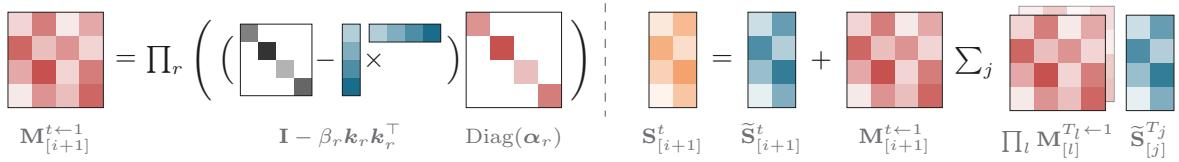
\includegraphics[keepaspectratio,alt={image}]{images/09812ec55031c337c687979b0afd3796d31459af1212ac73bbc4fac15d47d459.jpg}}

其中 \(\mathbf { M } _ { [ i + 1 ] } ^ { t  1 }\) 表示前 t 个本地 token 的累积转移。第一项包含本地 token 生成的状态，而第二项则通过本地 KDA 更新传播来自前序 rank 的上下文。在 \(t = T _ { i + 1 }\) 处，两个量 \(\mathbf { M } _ { [ i + 1 ] } ^ { T _ { i + 1 }  1 }\) 和 \(\widetilde { \mathbf { S } } _ { [ i + 1 ] } ^ { \mathbf { \Upsilon } _ { T _ { i + 1 } } }\) 都可以仅使用本地 token 计算，在 \({ \bf S } _ { [ i ] } ^ { T _ { i } }\) 可用之前完成，它们是每个 rank 与其他 rank 交换的片段。

公式 17 中的求和表明，每个状态完全由本地计算的片段组成。这些 rank 级更新满足结合律，因此每个 rank 的进入状态可以通过前缀扫描恢复 {[}77{]}。每个 rank 首先本地计算 \(\mathbf { M } _ { [ i ] } ^ { { \dot { T } } _ { i } \gets 1 }\) 和 \(\widetilde { \mathbf { S } } _ { [ i ] } ^ { T _ { i } }\)，然后通过一次 all-gather 交换这两个张量 \({[}1 3 9 ] . ^ { 2 }\)。在 all-gather 之后，rank \(i + 1\) 通过按顺序处理同一文档的前序片段，从 \(\mathbf { S } = \mathbf { 0 }\) 开始，在每个片段处应用 \(\mathbf { S } \gets \mathbf { M } _ { [ j ] } ^ { T _ { j }  \mathrm { i } } \mathbf { S } + \widetilde { \mathbf { S } } _ { [ j ] } ^ { T _ { j } }\)，从而重建 \(\dot { \mathbf { S } } _ { [ i ] } ^ { T _ { i } }\)。因此，KCP 仅需固定大小的 all-gather 用于循环状态同步，并实现线性计算扩展。

\subsection{3T 级预训练基础设施}\label{infra-for-3t-class-pre-training}

Kimi K3 预训练结合了带有虚拟阶段（VP）的流水线并行 \(( \mathrm { P P } )\) {[}48, 81{]}、专家并行（EP）{[}66{]}、ZeRO-1 数据并行 {[}100{]}、流水线 ZeRO-2 梯度分片 {[}145{]} 以及上下文并行（CP，§5.1.2）{[}50{]}。

\pandocbounded{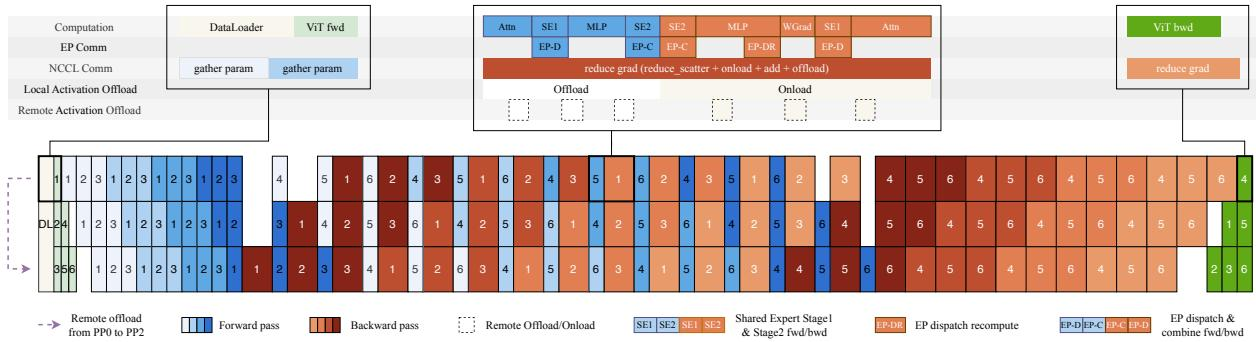
\includegraphics[keepaspectratio,alt={image}]{images/99383f1054624a8b730799bd7abdc5060108b3858086a1295d6844ecd2ad7775.jpg}}

图 11：计算、通信与卸载在不同 PP 阶段中的重叠。

MoE 层采用跨 EP rank 复制的共享专家，专家分发和合并的 all-to-all 通信与计算重叠以隐藏其延迟。

3T 级的原生多模态预训练面临三个关键问题：（i）token 负载在 EP rank 之间不均衡；（ii）激活值、梯度和优化器状态超出内存预算；（iii）视觉编码器高度可变地计算暴露在关键路径上。以下小节依次解决这些问题：完美均衡的专家并行 MoE 训练（§5.2.1）、内存高效训练（§5.2.2）以及多模态编码器优化（§5.2.3）。图 11 展示了由此产生的执行调度。

\subsubsection{完美均衡的专家并行 MoE 训练}\label{perfectly-balanced-expert-parallel-moe-training}

在传统 EP 方案中，token 负载在 rank 之间不均衡。由此产生的计算不均衡降低了训练吞吐量，而路由专家激活值的动态变化形状则导致严重的内存碎片。因此我们提出了 MoonEP3，一种通过动态冗余专家实现完美负载均衡的 EP 方案。MoonEP 保留了 DeepEP {[}147{]} 等传统方案的总体计算流程，同时额外引入了冗余专家的在线规划与迁移。在前向传播中，我们从当前 micro-batch 和层的路由器输出中规划冗余专家，并在路由专家计算之前预取它们。在后向传播中，我们将它们的梯度暂存到一个本地 reduce 缓冲区中，计算完成后将其 reduce 回其归属 rank 的梯度缓冲区。

有界冗余专家下的完美均衡。MoonEP 要求每个 rank 恰好接收 S K 个 token，其中 S 是序列长度，K 是每个 token 选择的专家数，从而所有 rank 执行相同量的计算。关键问题是多少冗余专家足以保证这种均衡。设 E 为专家数，R 为 EP 大小。我们证明，每个 rank 至多 E/R 个冗余专家总是存在一个均衡方案，且此上界本质上是紧的（§ E）。因此，每个 rank 预留 E/R 个冗余专家槽位即可保证规划总是有可行解，训练不会中断。相比之下，之前的工作如 ECHO {[}137{]} 和 UltraEP {[}132{]} 预设冗余专家数量或施加每个 rank 的 token 上限。当上限内不存在可行方案时，训练被迫停止，而上限本身需要手动调优，却仍残留不均衡。

在线规划。在每个训练步计算精确最优解的代价过高。因此，我们通过整数线性规划（ILP）为代表性情况离线计算精确解作为参考，并设计了一个 GPU 规划 Kernel，它近似最优、开销可忽略，且始终遵守 E/R 上界。

零拷贝通信。完美均衡也简化了通信路径。我们实现了一个融合的 permute/unpermute 算子，其中规划 Kernel 预先计算每个 token 的目标位置，因此 token 被直接发送到远程 rank 上按专家分组的位置，通信缓冲区的视图直接返回给计算，消除了中间拷贝。在最坏的不均衡情况下，支持同样零拷贝数据路径的 DeepEP 需要一个大小为 \(S \times K \times R\) 的通信缓冲区，而 MoonEP 由于完美均衡仅需一个固定的 \(S \times K\) 缓冲区。

静态形状下的免同步执行。在传统 MoE 实现中，每个专家的 token 数随训练步和层而变化，主机必须在每一层与设备同步以获取实际计算形状，才能启动专家计算，这导致管道在层间停顿。在完美均衡下，每个 rank 恰好接收 \(S \bar { \times } K\) 个 token，所有层的计算形状静态可知。这消除了每层 MoE 的主机同步，并缓解了主机端的 Kernel 启动开销。

Expert-GEMM 调度与重叠。即使整体负载在 rank 间完美均衡，每个 rank 内部的各专家 token 数仍不均衡，固定顺序、对工作负载无感知的调度会将这种不均衡转化为 SM 工作器之间不均衡的 makespan。因此，我们采用工作负载感知的调度器来调度路由专家 GEMM，该调度器在启动前根据当前 token 分布自适应调整参数，并在执行期间保持固定。一个轻量级启发式方法使用硬件指标的分析成本模型来选择这些参数，关键系数通过离线自动调优进行标定。对于共享专家，我们将其 GEMM 分发到单独的流上，以便与其他 Kernel 重叠。

\subsubsection{内存高效训练}\label{memory-efficient-training}

统一激活值管理器。我们设计了一个统一的激活值存储抽象，其中为后向传播保存的每个张量与一个可插拔的存储后端关联。重计算、量化和卸载/远程卸载在此抽象下仅是存储策略，可在张量粒度上自由组合；策略通过张量上的轻量级注解声明，与模型代码完全解耦。重计算以函数粒度执行，支持跨层重计算。在我们的实现中，所有 GPU 内存都在主计算流上分配，并在单一内存池中管理，避免了多流碎片化和主机端开销；激活值按层粒度预取回来并与计算重叠，引入的额外开销可忽略不计。在 Kimi K3 中，大部分激活值使用块级 FP8 量化 {[}58, 30{]} 结合卸载/远程卸载，逐元素算子则配置为重计算。

内存高效 MoE。在原生的 MoE 实现中，置换后 probs 的梯度计算依赖于前向输出 output。受 SonicMoE {[}41{]} 启发，我们通过数学变换将该梯度重写为仅依赖于中间激活 act\_output 和上游梯度 doutput 的形式，消除了对 output 的后向依赖，代价是增加一次额外的轻量级逐元素计算。此外，在分组 GEMM 的前向传播中，我们仅保存 dispatch 操作的输入；在后向传播期间，分组 GEMM 的输入通过重新计算 dispatch 来恢复。如图 11 所示，该重计算引入的通信可以与分组 GEMM 后向计算的一部分重叠，从而以可忽略的代价消除了这部分激活值存储。

内存高效 Attention Residual。对于 attention residual，我们设计了一个基于 Block AttnRes 的配套优化。块表示在边界层生成一次，并由所有后续层共享，直接驻留在 GPU 上。AttnRes 计算完全通过 checkpointing 包裹，因此每层为后向传播保存的激活值与标准残差架构相同。对于流水线并行，我们采用基于缓存的流水线通信 {[}57{]}，其中只有新生成的块在阶段之间增量传输，并在 micro-batch 完成后立即释放，达到内存占用的理论下界。

跨 PP rank 的激活值均衡。在交错 1F1B 流水线并行下，由于流水线预热，激活值在 PP rank 之间分布不均匀，驻留激活值的数量随 PP rank 增加而减少。为避免显存不足（OOM）错误，我们使用 Mooncake Transfer Engine {[}96{]} 将激活值远程卸载到其他 PP rank 的内存中，实现跨 PP rank 的激活值内存均衡。

流水线 ZeRO-2 梯度分片与卸载。除激活值外，我们使用流水线 ZeRO-2 梯度分片 {[}145{]} 在数据并行（DP）rank 之间分片梯度。此外，我们将分片后的梯度存储在 CPU 内存中，以降低 GPU 内存峰值使用量，同时在 GPU 上保留双梯度缓冲区。梯度在 DP rank 之间 reduce 进入双梯度缓冲区后，被累积到 CPU 分片中。

基于 P2P 的 Muon 正交化。分布式优化器将参数在 DP rank 之间均匀分片，而 Muon 中的 Newton--Schulz 正交化需要完整的参数矩阵，因此在每次更新前需要一个通信步骤来收集完整参数。原始方法在每个 rank 上对整个参数缓冲区执行 all-gather {[}73{]}，这不仅产生了巨大的内存占用，更使通信成为大规模下的主要瓶颈。取而代之，每个 rank 通过与其对应归属 rank 的点对点（P2P）通信，仅获取其本地拥有参数的各个分片，消除了完整参数缓冲区，同时降低了内存使用和通信量。通信和计算进一步以模型块缓冲区的粒度流水线化，隐藏了通信开销。

\subsubsection{多模态编码器优化}\label{multimodal-encoder-optimization}

多模态编码器中的动态 CP。在长上下文多模态训练中，大尺寸图像和长视频显著增加了视觉编码器的计算时间，并导致设备间严重的负载不均衡。为解决此问题，我们将上下文并行扩展到这些大样本上。单张大图像沿 patch 维度跨多个设备划分，注意力通过跨 CP rank 收集 key--value 对（gather-KV）来计算。此外，我们将每个 CP 组划分为若干子 CP 组，并以负载均衡的方式在它们之间分发多张大图像，防止通信比例随规模增长。这同时降低了大视觉样本的编码器延迟和跨设备负载不均衡，使得剩余的编码器计算能够隐藏在流水线气泡中。

PP 气泡中的编码器计算。在 Kimi K2.5 中，我们引入了分离编码器进程（DEP）{[}59{]}，将 ViT 和文本训练拆分为独立阶段，并在 PP 阶段之间平衡视觉的前向和后向传播。我们观察到，在交错 1F1B 流水线调度下，第一批 PP micro-batch 的文本前向传播全部在最开始调度，而最后一批 PP micro-batch 的文本后向传播在最末尾才完成。因此我们进一步分解 ViT 计算。第一批 PP micro-batch 的 ViT 前向传播在前期同步执行，其余前向传播被调度到流水线气泡中，后向传播也类似处理。结果，大部分 ViT 计算被隐藏在流水线气泡中，基本消除了视觉编码器的有效开销。

\subsection{百万 Token 智能体强化学习基础设施}\label{infra-for-1m-agentic-rl}

在有限的计算预算下，为 Kimi K3 这样的大模型将智能体强化学习扩展到百万 Token 上下文，使得资源效率成为首要目标。这推动了两项互补的工作：1）高效的训练和 rollout，包括 KV 缓存管理、请求调度和训练状态放置；2）用于长时交互的高性能可恢复沙箱。

\subsubsection{长上下文强化学习基础设施}\label{long-context-rl-infrastructure}

我们采用共置 RL 训练 {[}58{]} 将每个百万 Token 上下文的 Kimi K3 RL 实验控制在数百张 GPU 以内，并使用 partial rollout {[}118{]} 来降低超长轨迹的尾部延迟。这一设计实现了良好的硬件利用率，但也引入了 rollout KV 缓存（需要为下一次迭代保留）与训练所需内存之间的占用竞争。这一挑战在长上下文 RL 中更为严峻。

外部 KV 缓存池。在百万 Token 上下文的多步 rollout 中，前缀 KV 缓存未命中的代价极高。Partial rollout 在每次迭代开始时加剧了这一问题，因为来自上一迭代的许多未完成的长预填充请求同时到达。推测解码进一步加快了在相对固定的工具调用间隔内的请求周转，增加了前缀块的更替。这些问题可能触发抢占并降低缓存命中率，这对长上下文 RL 至关重要。

因此，我们通过写回设计将前缀保留与 GPU 驻留解耦。活跃的解码块保持在 GPU KV 缓存中，而可复用的空闲前缀仅在从 GPU 淘汰时才写回 CPU DRAM 中的外部 KV 缓存池，并在下次复用前预取回来。KDA 状态与相应的 MLA KV 缓存块一起卸载和预取，保持二者生命周期一致。与写通策略相比，此策略仅对离开活跃解码路径的前缀产生 CPU DRAM 使用和传输带宽，避免了仍在 GPU 上驻留且活跃的块的冗余 CPU 拷贝。

为了给外部缓存池提供足够的 DRAM，我们在训练迭代完成后将训练状态（模型权重和优化器状态）卸载到 NVMe。在 rollout 迭代之后，释放缓存池以避免与训练工作负载竞争。

Rollout 自动节流调度器。在多步 rollout 中，上下文随轨迹推进而逐步增长，使得基于全轨迹平均长度的固定并发度既难以估计，又在早期过于保守。反之，将并发度设置过高则会在后期产生 KV 缓存压力，并可能触发抢占。因此，我们在 LLM 请求调度层设计了一种自动节流机制，利用活跃请求数、排队请求数和 KV 缓存利用率等运行时信号，动态控制发送到推理引擎的请求数量。这使得早期 rollout 保持良好利用率，同时随着 KV 缓存压力上升降低并发度，无需手动调优即可避免欠饱和与过载。

非策略模型前向传播的梯度缓冲区复用。RL 损失计算通常需要仅前向的非策略模型，如参考模型，其权重过大无法常驻 GPU。我们将这些权重保留在 CPU 内存中，仅在需要时才实例化，将其参数张量托管在策略模型的 FP32 梯度缓冲区存储上。这复用了现有 GPU 内存，无需额外分配或引入碎片，并且由于真实梯度后续计算时会覆盖这些缓冲区，因此是安全的。

配合 ZeRO-2 梯度分片与卸载（§ 5.2.2），在 Kimi K3 RL 训练中，每个 GPU 仅为两个 VPP chunk 保留梯度缓冲区。我们将参考权重逐块流式加载到这些槽位中：一个槽位用于当前前向计算，另一个在预取下一个 chunk，从而在不增加 GPU 内存的情况下隐藏拷贝开销。

\subsubsection{沙箱基础设施}\label{sandbox-infrastructure}

我们部署了多个沙箱运行时来支持 Kimi K3 后训练和评估的多样化需求，包括传统的基于容器的运行时、GPU 沙箱运行时，以及最重要的一个——一种新的基于 microVM 的沙箱运行时 AgentENV。

AgentENV4 是与我们的合作伙伴联合开发的，专门为智能体 AI 工作负载设计的沙箱系统。它围绕三个核心设计目标构建：

• 高保真隔离沙箱运行时。随着智能体能力增强和任务难度提升，它们倾向于更激进地探索，甚至可能尝试 reward hacking。一方面，这带来了独特的安全挑战：在我们早期使用传统基于容器的沙箱运行时的实验中，观察到多次由非预期的智能体操作引发的内核 panic 和死锁。另一方面，我们希望尽可能允许探索，以免限制智能体的能力，而复杂任务需要一个接近真实环境的沙箱——例如，智能体应能挂载磁盘、运行容器，甚至随意启动虚拟机。通过使用 Firecracker {[}3{]} 运行隔离的 microVM，AgentENV 提供了基于容器的运行时无法匹敌的隔离度和保真度。

• 面向智能体 RL 的灵活沙箱生命周期。在底层，AgentENV 支持沙箱状态的增量 checkpoint 和恢复，其中 checkpoint 时仅保存自上次 checkpoint 以来被修改的内存页，checkpoint 和恢复延迟分别低至 133 ms 和 49 ms。在此基础上，AgentENV 提供了三个有助于提高智能体 RL 效率的高层操作。（a）暂停与恢复：暂停的沙箱不消耗内存或 CPU 资源；因此沙箱可以在智能体等待模型推理结果时暂停，这期间可能占沙箱生命周期的 98\%。（b）Fork：fork 从原始沙箱的精确状态创建一个新沙箱，同时保持原始沙箱继续运行，这对于无副作用的奖励评判非常有用。（c）快照：沙箱快照可以按固定间隔保存，用于错误恢复。

• 高效率与高密度。在我们的工作负载中，数万个沙箱（每个配备一组独特的镜像）可能需要在几秒钟内创建。我们采用 OverlayBD {[}68{]} 作为镜像格式，配合定制的 ublk 驱动实现、存储层共享和 P2P 传输，实现了大规模下的亚秒级启动延迟。我们通过写时复制内存和页面缓存优化进一步降低内存使用，在实际工作负载中取得高达 6.5 倍的内存超分比。

在 Kimi K3 的训练和评估过程中，共创建了 51,219,741 个沙箱，涉及 1,505,678 个镜像。

\subsection{推理与在线服务}\label{inference-and-online-serving}

为 Kimi K3 提供服务从生产侧暴露出同样的挑战：混合 KDA--MLA 架构维护两种本质不同的缓存，必须在百万 Token 上下文中联合管理；其新模块和高度稀疏的专家要求为每个模块定制 Kernel；而生产流量混合了单请求成本跨越三个数量级的请求。以下设计在三个层面应对这些挑战。在引擎层面，KDA 感知的前缀缓存将固定大小的循环状态打包到与 MLA KV 缓存相同的分页池中，并使长前缀可在请求间复用。在设备层面，为 KDA 解码、Block AttnRes 和稀疏潜在 MoE 定制的 Kernel 最小化每 token 延迟和内存流量。在集群层面，缓存感知的亲和调度和基于预算的准入控制将这些效率转化为可预测的服务。

\subsubsection{KDA 感知的前缀缓存管理}\label{kda-aware-prefix-cache-management}

Kimi K3 中的混合架构使前缀缓存复杂化：KDA 循环状态和 MLA KV 缓存在大小和生命周期上有本质区别，但缓存的前缀只有在二者能在同一边界上一起恢复时才可复用。因此，我们设计了一个 KDA 感知的前缀缓存，将两种缓存类型联合管理——从统一的分页布局到细粒度前缀复用，再到并发调度下的一致性——使得百万 Token 前缀的保留成本低廉并可在请求间复用。

混合 KDA--MLA 注意力的统一缓存布局。每个 Kimi K3 块由三层 KDA 和一层 Gated MLA 组成，其缓存在本质上有区别。MLA KV 缓存随序列长度增长，并按 token 分页；而 KDA 循环状态大小固定，每个请求只有一个拷贝。为每种缓存维护独立的管理器会重复分配、淘汰和传输逻辑。因此，我们将 KDA 状态打包到与 MLA KV 相同的分页块池中，将页面统一为相同的字节大小，使得两种页面类型共享同一套分配、引用计数和淘汰实现。在页面内部，所有 head 的状态按 head 依次连续存储，使得每个 head 的字节流自包含，并作为跨节点传输的最小单元。在预填充/解码分离部署下，当预填充和解码节点采用不同的 TP 度时，在传输路径上执行重新布局，GPU 端无需重新排布。这种非对称性在开发过程中证明很有用：任何类型混淆的访问会产生垃圾数据而非看似合理的数据——一种对池化布局的零开销健全性检查。

KDA 前缀缓存优化。基于块哈希的前缀缓存以一个物理块为粒度复用 KV 缓存：只有完整块才被哈希，因此只有块对齐的前缀才可复用。

这种耦合在 Kimi K3 中失效了。块哈希匹配要求所有层共享一个块大小，且前缀命中文仅在命中边界处的 KDA 状态已被持久化时才可复用。KDA 层每个序列维护一个大的循环状态而非逐 token 条目，因此状态快照仅在稀疏的边界处可行；共享块大小因此被迫设为 1024--6144 个 token——并且，由于哈希绑定到存储块，哈希粒度也被迫绑定，尽管 MLA 的逐 token 条目本身就允许更细的块。在如此粗的粒度下，前缀缓存几乎无用：短于一个块的请求永远无法被复用，分块预填充在跨越完整的块边界之前不能导出任何可缓存的前缀。

\pandocbounded{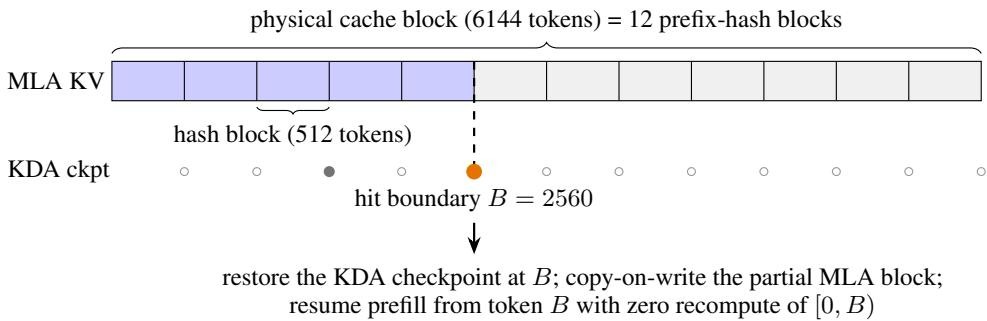
\includegraphics[keepaspectratio,alt={image}]{images/46b3dc78741e4634c7eda5bcddd443d6ff1c5e7bc4f43abfc8e0164324f3c3f7.jpg}}

图 12：物理缓存块内的细粒度前缀缓存。一个 6144 token 的物理块包含十二个 512 token 的哈希块，缓存的 MLA 块以蓝色显示，空块以浅灰色显示。下方的标记显示每个哈希边界处的 KDA checkpoint 状态。空心圆圈（）表示无存储 checkpoint 的边界，灰色圆点（）表示持久化的 KDA checkpoint，橙色圆点（）标记在 B = 2560 处的 checkpoint 命中。持久化的 checkpoint 是稀疏的，通常与对话轮次边界一致。该请求复用五个 MLA 哈希块和 B 处的 KDA checkpoint，然后恢复预填充，无需重新计算 [0, B)。

因此，我们将两种粒度解耦。前缀哈希以细粒度哈希块（例如 512 token）在 MLA 页面内部运行，而物理块保持为粗粒度的分配单元。KDA 的对齐方向相反：循环状态的 checkpoint 仅在 MLA 哈希端点的（一个稀疏子集）处保存——这是查找唯一能引用的位置。

在预填充期间，部分填充的 MLA 页面以其最后完整哈希块的链式哈希注册到前缀缓存索引中，其中每个哈希覆盖其之前的所有哈希块，因此匹配一个端点即验证了到该点为止的整个前缀；注册端点随页面填充而推进。同时，在每次前向传播后，KDA Kernel 在处理的最后一个哈希对齐位处持久化循环状态。Checkpoint 较大，因此随请求推进而被取代的中间 checkpoint 会被回收，而对话轮次边界处的 checkpoint 则保留用于跨请求复用。缓存的 checkpoint 是只读快照：命中时通过在下一次前向传播之前拷贝到请求的私有运行状态中来恢复状态，新的 checkpoint 写入新的槽位，因此对其他请求可见的 checkpoint 永远不会被就地修改。

查找分两个阶段进行（图 12）。MLA 阶段通过链式哈希匹配完整物理块，在第一个缺失块处，回退到其内部的哈希端点，使部分填充的页面仍可命中。然后，KDA 阶段要求候选边界处在每个 KDA 缓存组都有一个 checkpoint，每个缓存组维护一个独立的循环状态。命中是同时满足两个阶段的最长边界——始终是哈希块的倍数，且不要求是物理块的倍数。在图 12 中，一个前 2800 token 与缓存前缀匹配的请求在 \(\dot { B } = 2 5 6 0 = 5 \times \dot { 5 } 1 2\) 处命中，深入到一个 6144 token 物理块内部，并从 token B 处恢复预填充，而无需重新计算 [0, B)。

并发调度下的一致性。其余设计要点均由共享部分填充块的具体失败模式决定：在这种场景下，一个命中块既是共享缓存条目，又是私有请求的增长点；MLA 和 KDA 缓存组必须在每个命中边界上达成一致。首先，所有缓存组从一个共享的空闲列表中获取块，因此为一个组分配私有拷贝可能淘汰另一个组刚刚命中的块；因此，每个命中块在分配任何内容之前，都会在所有组之间被钉住。其次，向私有块的拷贝在当前调度步内紧接前向传播之前在 GPU 上执行，因此当前调度步内分配或注册的块仍可能将前一个拥有者的字节传递给读者；此类块在拷贝落地之前被排除在匹配之外。第三，一个 checkpoint 只有在每个 KDA 组都存在时才能恢复请求，因此淘汰一个组的 checkpoint 原子性地使其兄弟 checkpoint 无效——一个 checkpoint 要么在所有组都可命中，要么在任何一个组都不可命中。通过这些机制，每个已注册状态始终精确对应其声明的 token 前缀，混合 KDA--MLA 模型的前缀缓存达到了与全注意力模型同样的通用性：任何共享前缀在任何 512 token 边界处都可复用，与请求长度、分块或调度交叠无关。

\subsubsection{高性能 Kernel}\label{high-performance-kernels}

Kimi K3 引入了几个新的架构模块：KDA（§2.1.1）、Block AttnRes（§2.2）和 Stable LatentMoE（§2.3）。我们为每个模块优化了 Kernel 实现。

KDA。与 KDA 预填充（§5.1）相比，KDA 解码呈现一组不同的挑战：主要瓶颈从利用并行性转变为高效管理不断演化的循环状态，该状态在每个解码步都被就地更新。这种就地更新在基于 MTP 的推测解码中变得棘手：如果验证拒绝了一个子集的草稿 token，状态已经推进到最后一个被接受 token 之后，无法简单回滚。为每个草稿位维护状态快照可以实现回滚，但也会倍增状态流量——这一代价在在线服务典型的较大批次下占主导地位。

然而，任何被接受的草稿前缀之后的状态完全由草稿 token 的投影输入决定，这些输入远小于状态本身。因此，我们仅缓存这些投影输入，在芯片上重建被接受 token 的状态，并写回已验证 token 和 bonus token 的状态，这一设计与同期工作 ReplaySSM {[}25{]} 独立提出。重放的 token、bonus token 和下一个草稿窗口在单个融合 Kernel 内共享一个循环循环，覆盖短卷积、输入归一化、门控、KDA 循环和输出归一化。验证延迟随验证 token 数呈亚线性增长，并保持在状态缓存基线的延迟之下。由于投影缓存从不离开解码阶段，前缀缓存和预填充-解码分离在非推测推理中操作相同的负载。

Block AttnRes。Block AttnRes {[}57{]} 遵循两阶段调度：批量跨块传播每块读取一次缓存的块表示，之后每层通过 online-softmax 合并 {[}79{]} 融入块内部分和。在预填充和解码中，内存访问占这些 Kernel 成本的很大一部分，因此我们两个阶段的优化都主要集中在内存效率上。

对于预填充，在每个张量并行（TP）rank 上实例化块表示会产生大量冗余的内存消耗。因此，我们对激活值采用序列并行（SP）：将 TP all-reduce 分解为 reduce-scatter 和 all-gather，块内 Kernel 插入在两次集合通信之间，对序列分片的隐藏状态进行操作，使得每个 token 的块表示恰好在一个 rank 上实例化。这消除了额外的内存消耗，并降低了预填充期间 Block AttnRes 的 I/O 开销。

对于解码，我们在旁路流上启动跨块 Kernel，使其与主流上的独立计算重叠。块内 Kernel 则通过融合来精简：将 AttnRes 输出与其部分和更新的合并，以及后续的 RMSNorm，融合到前序的 TP all-reduce 中，从而消除了块内阶段的专用 Kernel。这些优化共同隐藏了跨块传播的延迟，并降低了块内阶段的内存流量。

Stable LatentMoE。Stable LatentMoE 同时增加了专家的总数和每个 token 激活的专家数。专家空间和每 token 专家数的增长提高了调度和协调开销，使得传统 MoE Kernel 难以维持高硬件利用率。这些挑战推动了对该模块的专用 Kernel 优化。

为缓解潜在 GEMM 的开销，我们采用了三项优化。首先，将潜在下投影与 MoE 路由器融合为单个 GEMM。其次，跨 rank 分片潜在权重矩阵，并使用 multimem store 指令将输出 all-gather 融合到 GEMM epilogue 中。最后，将由此产生的通信与其他算子（如共享专家计算）重叠。这些优化共同消除了冗余权重流量和重复计算，同时将通信延迟隐藏在计算之后。

对于路由专家，在小批次下，分组 GEMM 退化为对权重矩阵的内存受限流式访问——对于这种场景，传统的以 tile 为中心的 Kernel 由于其面向计算的设计和预处理开销而不适用。我们改为基于 WarpDecode {[}12{]} 的以 token 为中心的设计构建 MoE 解码 Kernel，其中每个 warp 负责一个输出神经元，直接从内存流式读取相关权重。为进一步提高并行度，我们将每个 warp 细分为更细粒度的 lane 组，每组处理一个不相交的专家子集，随后进行 warp 级的部分结果归约。此外，权重布局通过一次性预处理代价进行离线置换，大幅降低了运行时的反量化开销。

\subsubsection{集群级调度}\label{fleet-level-scheduling}

在单个推理实例之上，挑战从单请求效率转变为可预测性：一次前缀缓存未命中的代价比命中高出数个数量级，而百万 Token 请求的突发流量可能饿死短请求。我们提出两项集群级调度策略来应对：缓存感知的亲和调度将每个会话路由到持有其前缀缓存的集群，同时限制集群故障的代价；基于预算的准入控制为每个请求类分配各自的资源预算，使得突发的长上下文流量不会降低系统整体的 SLO。

缓存感知的亲和调度。在百万 Token 上下文中，典型的编码输入携带 400K token 的前缀，但只需要 4K token 的预填充增量，因此一次前缀缓存命中避免了重新预填充整个前缀，代价比未命中低数个数量级。因此，我们将每个请求路由到持有其前缀缓存的集群，因为将缓存转移到另一个集群需要通过远比集群内部网络慢的跨集群链路。然而，这种缓存感知的亲和性将每个会话绑定到单个集群，该集群的故障会中断所有绑定到它的会话。因此，一致性哈希将每个会话钉在两个集群上：一个主集群为其提供服务，一个预先分配的备用集群在主集群故障时接管。备用集群不持有该会话的任何前缀缓存，必须在故障切换时重新预填充。由于一致性哈希将不同会话的备用分配均匀分布在整个集群中，重新预填充的工作被分摊到多个集群而非集中在一个集群上。因此在常见情况下保留了缓存局部性，同时任何单集群故障的影响保持受限。

基于预算的准入控制。生产流量混合了 2K token 以下的短请求与高达百万 Token 的超长请求，因此单请求成本跨越约三个数量级，任意固定数量的请求所产生的总负载高度不可预测。基于"平均请求"的容量规划、排队模型和速率限制配额在这种方差下全部失效。在一个典型故障模式中，一波长上下文请求突发流量耗尽可用计算资源，随后到达的短请求无法被及时调度，导致所有流量的首 token 延迟（TTFT）恶化。因此，我们采用基于预算的准入控制，为不同的请求类分配独立的资源预算，使得突发的长上下文流量最多消耗其自身的容量份额，而不会降低其他请求类所体验的系统级 SLO。

